\documentclass{cours}

\title{Jeux et Automates\\ \small Plan Présentation LFCC}
\author{Matthieu Boyer}
\date{\today}

\usetikzlibrary{automata, arrows, calc, matrix}

\begin{document}
\begin{abstract}
    Dans ce rapport, on s'intéresse à des manières de représenter des jeux par la théorie des langages formels, en particulier par les automates et par les automates à pile. On présente alors une nouvelle caractérisation de la régularité d'un langage comme sa reconnaissance par une certaine représentation des jeux. Puis, en modifiant cette représentation, on trouve une caractérisation des langages algébriques par les jeux. Enfin, on s'intéresse à une manière de représenter le \textit{Game Design} par des automates en introduisant un délai sur les transitions, et on regarde quelques exemples d'applications.
\end{abstract}
\section*{Introduction}
Dans la suite on ne s'intéresse qu'à des jeux à plusieurs joueurs i.e. plus de deux.\\ Un jeu à plusieurs joueurs est, de manière informelle, une abstraction d'un jeu ressemblant par exemple à la belote : Chaque joueur, à son tour, va choisir, parmi un éventail de coups possibles, celui qu'il souhaite effectuer, modifiant alors l'état du jeu. En reprenant l'exemple de la belote, un coup est une carte de la main du joueur, qui ne sait pas exactement quelles cartes ont ses adversaires, et qui ne peut la jouer que sous certaines conditions, à résoudre dans l'ordre :
\begin{enumerate}
    \item Soit il est le premier à jouer
    \item Soit la carte est de la \textit{bonne} couleur
    \item Soit la carte est un atout plus grand que le dernier joué
    \item Soit la carte est une coupe (atout lorsqu'un autre couleur est jouée)
    \item Soit il ne peut rien jouer d'autre remplissant les conditions précédentes
\end{enumerate}
Il paraît alors raisonnable qu'en limitant les transitions possibles de l'état de jeu selon l'état et selon les règles du jeu, on puisse modéliser un jeu par un automate. Toutefois, le manque d'informations d'un joueur sur les mains de ses adversaires, semble aussi limiter la description directe du jeu avec un caractère non-déterministe.

\section{Jeux et Automates}

\subsection{Première définition de Jeu}
On introduit d'abord une première définition de jeu :
\begin{definition}
    Un jeu est un triplet $\left(P, A_{i}, \succeq_{i}\right)$ où $P$ est un ensemble de joueurs, $A_{i}$ est un ensemble d'actions pour le joueur $i \in P$ et $\succeq_{i}$ est une relation de préférence pour le joueur $i$.
\end{definition}

Pour le \textsc{Dilemme du Prisonnier}, on a par exemple : $P = \left\{0, 1\right\}$, $\forall i, A_{i} = \left\{A, N\right\}$ et $\succeq_{i}$ peut se décrire sur l'arbre de jeu suivant de manière numérique :
\begin{center}
    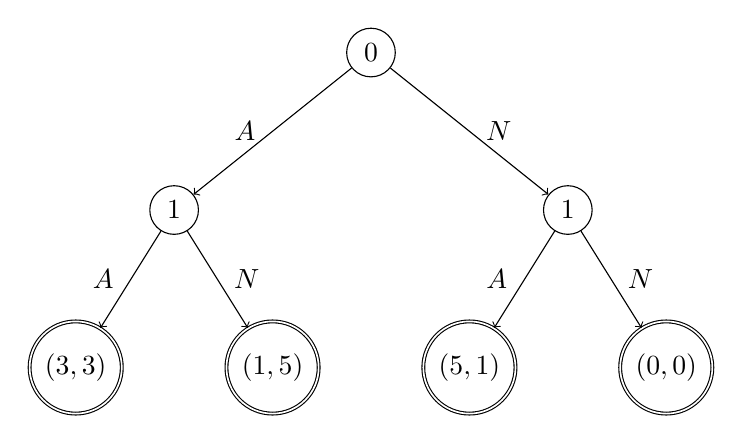
\begin{tikzpicture}[level distance=2cm,
            level 1/.style={sibling distance=5cm},
            level 2/.style={sibling distance=2.5cm}]
        \tikzstyle{every node}=[circle,draw]
        \node {0}
        child {node {1}
                child {node[double] {$(3, 3)$} edge from parent[->] node[left, draw = none] {$A$}}
                child {node[double] {$(1, 5)$} edge from parent[->] node[right, draw = none] {$N$}}
                edge from parent[->] node[left, draw = none] {$A$}
            }
        child {node {1}
                child {node[double] {$(5, 1)$} edge from parent[->] node[left, draw = none] {$A$}}
                child {node[double] {$(0, 0)$} edge from parent[->] node[right, draw = none] {$N$}}
                edge from parent[->] node[right, draw = none] {$N$}
            };
    \end{tikzpicture}
    \label{gametree:full_info_pridi}\\
    Arbre de Jeu du \textsc{Dilemme du Prisonnier} à information totale.
\end{center}

Ici, chaque noeud interne de l'arbre correspond à un joueur, chaque arête à un coup qu'il peut jouer, c'est-à-dire dans notre cas, choisir d'avouer ($A$) son crime, ou bien de le nier ($N$) et les feuilles de l'arbre représentent les résultats, cf. Table \ref{pridi:res_one}.\\
\begin{table}[ht]
    \centering
    \caption{Résultats du \textsc{Dilemme du Prisonnier}}
    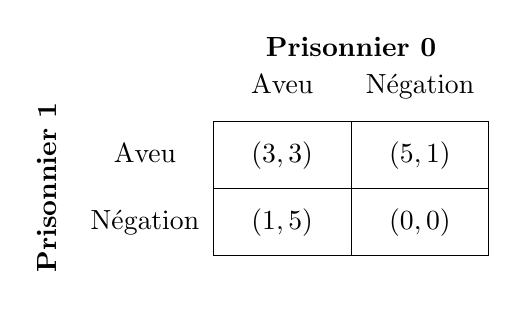
\begin{tikzpicture}[element/.style={minimum width=1.75cm,minimum height=0.85cm}]
        \matrix (m) [matrix of nodes,nodes={element},column sep=-\pgflinewidth, row sep=-\pgflinewidth,]{
        & Aveu & Négation \\
        Aveu & |[draw]|$(3, 3)$ & |[draw]|$(5, 1)$ \\
        Négation & |[draw]|$(1, 5)$ & |[draw]|$(0, 0)$ \\    };

        \node[above=0.25cm] at ($(m-1-2)!0.5!(m-1-3)$){\textbf{Prisonnier 0}};
        \node[rotate=90] at ($(m-2-1)!0.5!(m-3-1)+(-1.25,0)$){\textbf{Prisonnier 1}};
    \end{tikzpicture}
    \label{pridi:res_one}
\end{table}
\begin{definition}
    On appelle la description d'un jeu à information totale sous forme d'arbre précédente la description extensive de ce jeu.
\end{definition}

Toutefois, d'autre descriptions peuvent être préférables, notamment lorsque l'un des joueurs n'a pas d'information sur les coups des autres joueurs, comme c'est le cas dans certaines variantes du \textsc{Dilemme du Prisonnier}. En effet, on considérait ici que le prisonnier\footnote{NDA : \textit{I am not a number ! I am a free man !}} $1$ est informé du choix du prisonnier $0$, ce qui n'est pas un très bon choix de la part des gêoliers.
\begin{definition}
    On parle de jeu à information imparfaite (par opposition aux jeux à information totale ou jeux extensifs), lorsque le joueur actuel n'a pas d'informations sur les coups des joueurs précédents. On représente ceci en rajoutant sur l'arbre de jeu l'information possédée par un joueur lors de son coup en entourant l'ensemble des positions possibles.
\end{definition}

Dans le cas du \textsc{Dilemme du Prisonnier}, on modifie l'arbre \ref{gametree:full_info_pridi} comme suit :
\begin{center}
    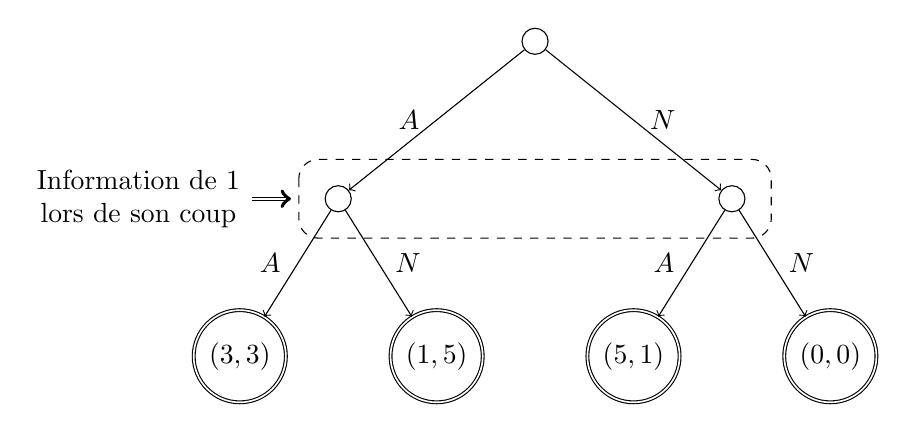
\begin{tikzpicture}[level distance=2cm,
            level 1/.style={sibling distance=5cm},
            level 2/.style={sibling distance=2.5cm}]
        \tikzstyle{every node}=[circle,draw]
        \node(0) {}
        child {node {}
                child {node[double] {$(3, 3)$} edge from parent[->] node[left, draw = none] {$A$}}
                child {node[double] {$(1, 5)$} edge from parent[->] node[right, draw = none] {$N$}}
                edge from parent[->] node[left, draw = none] {$A$}
            }
        child {node {}
                child {node[double] {$(5, 1)$} edge from parent[->] node[left, draw = none] {$A$}}
                child {node[double] {$(0, 0)$} edge from parent[->] node[right, draw = none] {$N$}}
                edge from parent[->] node[right, draw = none] {$N$}
            };
        \draw[dashed,rounded corners=7]($(0-1)+(-.5,.5)$)rectangle($(0-2)+(.5,-.5)$);
        \tikzstyle{every node} = []
        \node at ($(0-1) + (-1,.)$)[label ={[align = center]left : Information de $1$\\ lors de son coup}]{};
        \draw[->, double, distance = 5pt]($(0-1) + (-1.1,.)$)--($(0-1)+(-.6,.)$);
    \end{tikzpicture}
\end{center}
\begin{definition}
    Une partie sur un jeu est une suite d'états de ce jeu, ou, de manière équivalente, une suite de coups $s_{0}s_{1}\ldots s_{k}$ tels que : 
    \begin{itemize}
        \item $\forall i, s_{2i} \in A_{0}$ et $s_{2i + 1} \in A_{1}$.
        \item $\not{\exists} s_{k + 1} \in A_{i}$ où $i = 1$ si $k \equiv 0 \mod 2$ et $i = 0$ sinon.
    \end{itemize}
\end{definition}

\subsection{Les Automates vus comme des Jeux}
\begin{definition}
    Si $A = \left(Q, \Sigma, \delta, \iota, F\right)$ est un automate, on définit $G_{A}$ un jeu à deux joueurs $P_{1}$ et $P_{2}$. Dans ce jeu, $P_{1}$ joue des états de $Q$ et $P_{2}$ joue des lettres de $\Sigma$. Si $P_{1}$ joue $q \in \Sigma$ alors $P_{2}$ doit jouer $s$ tel que $\delta(q, s) \neq \emptyset$.
\end{definition}
On joue comme suit :
\begin{itemize}
    \item $P_{1}$ joue $q_{0}$ l'état initial.
    \item $P_{2}$ doit jouer une lettre $s \in \Sigma$
    \item La partie se termine lorsque $P_{1}$ joue un état de $F$ et que $P_{2}$ n'a plus de coup valable.
\end{itemize}

On va alors pouvoir définir formellement la notion de stratégie d'un joueur sur un tel jeu : 
\subsection{Information et Déterminisme}
\begin{itemize}
    \item Si $A$ est déterministe, $G_{A}$ est équivalent à un jeu à information parfaite, ou jeu extensif.
    \item Réciproquement, si $A$ n'est pas déterministe, on peut d'une meilleure manière définir des ensembles d'informations pour chacun des joueurs récursivement.
\end{itemize}

\subsection{Langage et Stratégies Gagnantes}
\begin{itemize}
    \item Une stratégie gagnante pour $P_{1}$ est une stratégie telle que $P_{1}$ a joué un état final et $P_{2}$ ne peut plus jouer.
    \item Une stratégie pour $P_{2}$ définie par $w \in \Sigma^{\star}$ est telle que $P_{2}$ joue les lettres de $w$ indépendamment de ce que $P_{1}$ joue.
    \item Une stratégie gagnante pour $P_{2}$ est une stratégie $w$ de longueur $n$ où $P_{1}$ n'a pas de coup valide.
    \item On note $S(G_{A})^{n}$ l'ensemble de ces stratégies, et $L(A)^{n}$ l'ensemble des mots de longueur $n$ reconnus par $A$. Alors, on prouve que $S(G_{A})^{n} = L(A)^{n}$.
\end{itemize}

\section{Jeux et Grammaires}
\subsection{Jeux Hors-Contexte}
\begin{itemize}
    \item Définition d'un Jeu par une Grammaire
    \item Définition de la Victoire d'un Jeu pour un mot (similaire à ce qui précède).
\end{itemize}

\subsection{Jeux et Systèmes à Pile}
\begin{itemize}
    \item Définition d'un Système à Pile comme un automate à pile sans entrée.
    \item Preuve qu'on peut construire un automate à pile de sorte qu'un joueur gagne le jeu $G, w$ si et seulement si le calcul sur $w$ de l'automate atteint un état $gagnant$ et réciproquement, qu'on peut construire un jeu à partir d'un automate à pile.
\end{itemize}

\subsection{Application aux Jeux de Cartes}
\begin{itemize}
    \item Description du Uno par une Grammaire.
\end{itemize}


\section{Game Design et Automates}
Je ne sais pas encore exactement à quel point aller loin dans ce sujet.
\begin{itemize}
    \item Définition des objets par des alphabets
    \item Représentation du fil du jeu par un automate dont les transitions sont liées aux actions du joueur.
\end{itemize}


\begin{thebibliography}{5}
    \bibitem{game-rep-automata} A-Games: using game-like representation for representing finite automatas \textit{Cleyton Slaviero, Edward Hermann Haeusler}
    \bibitem{card-game-lang} A Card Game Description Language \textit{Jose M. Font, Tobias Mahlmann, Daniel Manrique, and Julian Togelius}
    \bibitem{cfgames} Active Context-Free Games \textit{Anca Muscholl, Thomas Schwentick, and Luc Segoufin}
    \bibitem{game-desing-automata} Computing Game Design with Automata Theory \textit{Noman Sohaib Qureshi, Hassan Mushtaq, Muhammad Shehzad Aslam, Muhammad Ahsan, Mohsin Ali and Muhammad Aqib Atta}
    \bibitem{cfgames-sum} Summary for Context Free Games \textit{Lukáš Holík, Roland Meyer and Sebastian Muskalla}
\end{thebibliography}



\end{document}

